%UNIT 11: DAMPED AND UNDAMPED LINEAR SYSTEMS
%%%%%%%%%%%%%%%%%%%%%%%%%%%
%%%% Put the following at the top of each .tex file  %
\pagestyle{fancy}
\renewcommand{\theUnit}{11}
\ifthenelse{\isundefined{\UnitPageNumbers}}{}{\setcounter{page}{1}}
\rhead{Unit \theUnit: Damped and Undamped Linear Systems}
\lhead{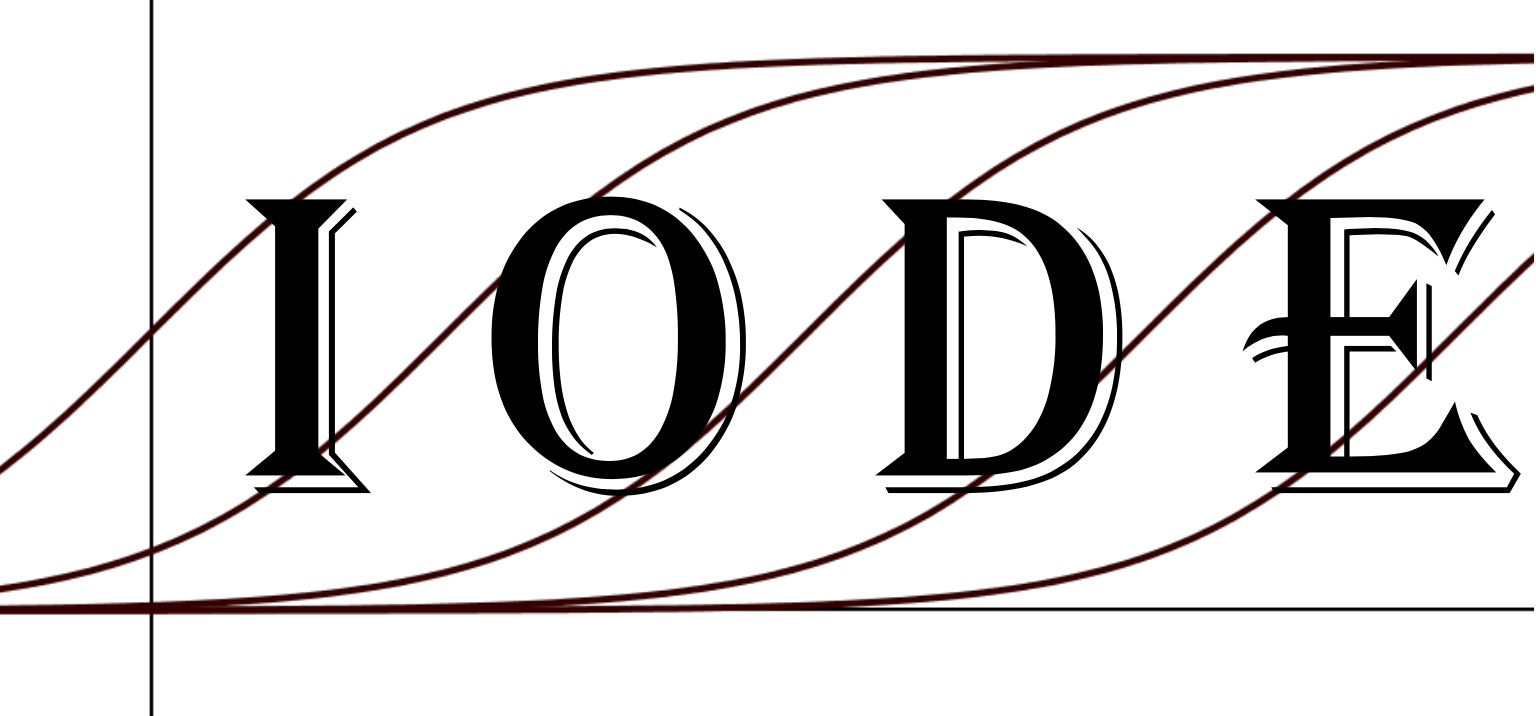
\includegraphics[width=1.25cm]{IODE-logo.png}}
\rfoot{\mypage}
\lfoot{}
\cfoot{}
\fancypagestyle{firstfooter}{\footskip = 50pt}
\renewcommand{\footrulewidth}{.4pt}
%%%%%%%%%%%%%%%%%%%%%%%%%%%
\vspace*{-20pt} \thispagestyle{firstfooter}
\pagebegin{Spiraling Solutions - Spring Mass Revisited}

In a previous problem we applied Newton's law of motion for a spring mass system and obtained the second order differential equation  $\displaystyle \frac{d^2x}{dt^2}+\frac{b}{m}\frac{dx}{dt}+\frac{k}{m}x=0$, where $x$ is the position of the object attached to the end of the spring, $m$ is the mass of the object, $b$ is the damping coefficient, and $k$ is the spring constant.
Using the fact that velocity is the derivative of position and choosing the mass $m = 1$ and the spring constant $k = 2$, we converted this to the following system of two differential equations:  
\begin{center}
\raisebox{1.5\height}{$\displaystyle \begin{aligned}
\frac{dx}{dt}&=y \\ \frac{dy}{dt}&= -2x-by
\end{aligned}$} \hspace{1in}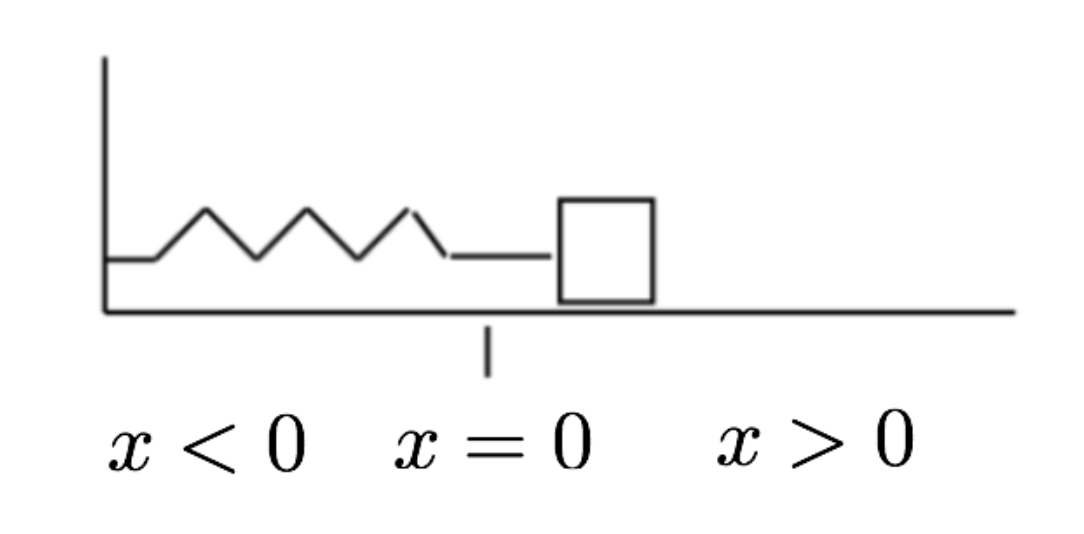
\includegraphics[width=2in]{11/11SpringMass.png}
\end{center}

We were able to figure out the $x(t)$ and $y(t)$ equations when the value of the friction parameter was such that there were straight line solutions in the phase plane. 
Such a situation is typically referred to as \textit{overdamped}. The situation is called \textit{damped} when the differential equations predict that the mass will oscillate about the 0 position and \textit{undamped} when there is no friction. 
In the following problems we figure out the $x(t)$ and $y(t)$ equations for the damped case. We consider the undamped situation in the homework. \\

The vector field for the case when $b = 2$ is shown below.  Based on this vector field, it appears that the differential equations predict that the mass will oscillate back and forth. 
%Even though there are not any straight line solutions, we can still use the same algebraic approach as before to get the $x(t)$ and $y(t)$ equations for any initial condition, but we will have to deal complex numbers. Problems \ref{11problem1}-\ref{11problem7} outline a way to do this.

\begin{center}
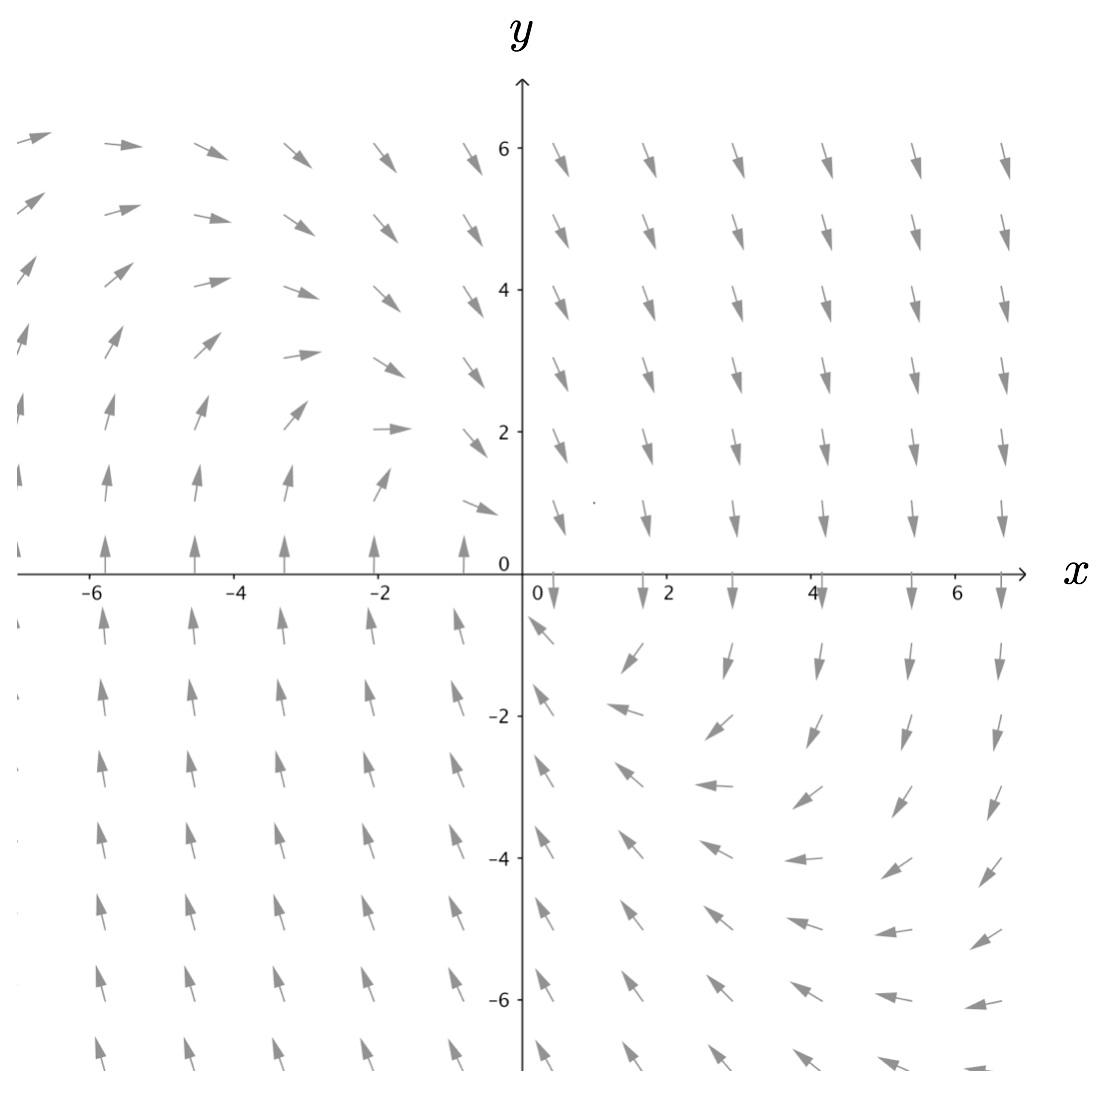
\includegraphics[width=3.5in]{11/11figure.png}
\end{center} 

You might recall that in a previous question, a student named Joey had set $b=2$ and found straight line solutions, and you were asked to confirm or explain why he was mistaken.  When you set $y=ax$ and solved for $a$, you found that the slopes were complex numbers, and so concluded that there were not any straight line solutions.  Nevertheless, a very similar technique to our previous work will allow us to take those complex-valued slopes and create real-valued solutions.  


\clearpage
So far, our technique for finding straight line solutions comprised the following steps:
\begin{enumerate}
\item Temporarily assume that we are on a straight line, so that $y=ax$ (or $\frac yx=a$).  Then, use $\frac{dy}{dx} = \frac{dy}{dt} / \frac{dx}{dt}$ to find the values of $a$ that are consistent with both equations.  
\item\label{line10} Having found one value for $a$, pose two initial value problems by using $y=ax$ to reduce $\frac{dx}{dt}$ to only be in terms of $x$, and $\frac{dy}{dt}$ to only be in terms of $y$.  Your initial conditions must also satisfy $y=ax$, so we can use an initial condition like $x(0)=1$, $y(0)=a$.
\item\label{goto10}Solve those linked initial value problems.  The solution functions $x$ and $y$ should be:
\begin{itemize}
\item exponential functions with the same exponent
\item still satisfy $y=ax$
\end{itemize}
The solutions satisfying those two properties are our ``straight line solution.'' 
\item\label{inserthere} Repeat steps \ref{line10}--\ref{goto10}, for the other slope $a$ to achieve a different straight line solution.
\item\label{generalsolution} Now you have two different (straight line) solutions which are pairs of functions $x_1(t)$ is paired with $y_1(t)$ and $x_2(t)$ is paired with $y_2(t)$.  We concluded that we could take any linear combination of these (straight line) solutions and still have a solution, so our general solution became $x(t)=c_1 x_1(t) + c_2 x_2(t)$ and $y(t) = c_1 y_1(t) + c_2 y_2(t)$.   
\item Use the general solution to solve an initial value problem, or make predictions about the long-term behavior of the system, or address other pertinent questions.

\end{enumerate}
What we will find is that we have a few additional steps after step \ref{inserthere}.  We first have to make two different real-valued solutions, and we can take linear combinations of these real-valued solutions to form the general solution, as in step \ref{generalsolution} above.

Consider again 
\begin{align*}
\frac{dx}{dt}&=y \\ \frac{dy}{dt}&= -2x-2y
\end{align*}
\begin{enumerate}
\item We suppose $y=ax$, so that $\frac{dy}{dx} = a = \frac{-2x-2(ax)}{ax} = \frac{-2-2a}{a}$.  
Therefore, $a^2 + 2a + 2 = 0$, and employing the quadratic formula, we find that $a = \frac{-2 \pm \sqrt{2^2 - 4\cdot1\cdot2}}{2} = -1 \pm i$.
\item Along the line $y=(-1+i)x$, we also have $x=\frac{1}{-1+i} y = \frac{-1-i}{-1-i}\cdot\frac{1}{-1+i}  y = \frac{-1-i}{(-1)^2 -i +i -(i)^2} y = \frac{-1-i}{1 + -(-1)} y = \frac{-1-i}{2} y$
Taking the initial conditions $x(0) = 1$ and $y(0) = -1+i$, we make the substitutions into $\frac{dx}{dt}$ and $\frac{dy}{dt}$:
\begin{align*}
\frac{dx}{dt}&=(-1+i)x ~~;~~ x(0) = 1 \\ \frac{dy}{dt}&= -2\frac{(-1-i)}{2}-2y ~~;~~ y(0) = -1+i
\end{align*}
Which simplifies to
\begin{align*}
\frac{dx}{dt}&=(-1+i)x~~ ;~~ x(0) = 1 \\ \frac{dy}{dt}&= (1+i)y -2y = y + iy - 2y = -y + iy = (-1+i)y~~ ;~~ y(0) = -1+i
\end{align*}
\item Solving these initial value problems by separation of variables (or inspection) gives us $x_1(t) = 1 e^{(-1+i)t}$ and $y_1(t) = (-1+i) e^{(-1+i)t}$.  We notice that $x(t)$ and $y(t)$ are exponential functions with the same exponent, and that $y=(-1+i)x$, so we are confident in moving forward.
\item Similarly, along $y=(-1-i)x$, we have $x= \frac{1}{-1-i} y = \frac{-1+i}{-1+i}\cdot \frac{1}{-1-i} y = \frac{-1+i}{2} y$.  Choosing an initial condition along $y = (-1-i)x$, say, $x(0) = 1$, $y(0) = -1-i$ and making the substitutions into the original differential equations yields:
\begin{align*}
\frac{dx}{dt}&=(-1-i)x ~~;~~ x(0) = 1 \\ \frac{dy}{dt}&= -2\frac{(-1+i)}{2}-2y ~~;~~ y(0) = -1-i
\end{align*}
Which simplifies to: 
\begin{align*}
\frac{dx}{dt}&=(-1-i)x ~~;~~ x(0) = 1 \\ \frac{dy}{dt}&= -2\frac{(-1+i)}{2}-2y = (1 - i)y - 2y = y-iy - 2y = -y-iy = (-1-i)y~~;~~ y(0) = -1-i
\end{align*}
And solving these by separation (or inspection) yields $x_2(t) = e^{(-1-i)t}$ and $y_2(t) = (-1-i)e^{(-1-i)t}$.  We notice that both are exponential with the same exponent, and that $y=(-1-i)x$ so we are confident to proceed.  
\item Now that we have two different ``straight line'' solutions, namely
 \begin{align*}
x_1(t) = e^{(-1+i)t} &\textrm{~~and~~} x_2(t) = e^{(-1-i)t}\\
y_1(t) = (-1+i)e^{(-1+i)t} &\textrm{~~and~~}  y_2(t) = (-1-i)e^{(-1-i)t}
\end{align*}
\end{enumerate}
 we have to deviate slightly from our original procedure.  We need to use Euler's formula: $e^{i\theta} = \cos(\theta) + i\sin(\theta)$.  From this, we note that $e^{(\alpha+\beta i)t} = e^{\alpha t + i(\beta t)} = e^{\alpha t} \cdot e^{i (\beta t)} = e^{\alpha t} \cdot (\cos(\beta t) + i \sin(\beta t))$.  Similarly, $e^{(\alpha - \beta i)t} = e^{\alpha t + i (-\beta t)} = e^{\alpha t} \cdot e^{i (-\beta t)} = e^{\alpha t}\cdot (\cos(-\beta t) + i\sin(-\beta t) = e^{\alpha t} \cdot (\cos(\beta t) - i\sin(\beta t)$.   

Applying $e^{(\alpha \pm \beta i)t} = e^{\alpha t} (\cos(\beta t) \pm i \sin (\beta t))$ to our ``straight line'' solutions, we have $\alpha =1$, and $\beta = 1$, so:
 \begin{align*}
x_1(t) = e^{-t}(\cos(t) + i\sin(t)) &\textrm{~~and~~} x_2(t) = e^{-t}(\cos(t) - i \sin(t))\\
y_1(t) = (-1+i)(e^{-t}(\cos(t) + i\sin(t)) &\textrm{~~and~~}  y_2(t) = (-1-i)e^{-t}(\cos(t) -i\sin(t))
\end{align*}
Now we have to roll up our sleeves and get our hands dirty with some algebra.  We must expand out the expressions for each of our solution functions, and collect together the real and imaginary parts.  
Distributing the $e^{-t}$ terms is all that we have to do for $x_1$ and $x_2$, and is a useful step for $y_1$ and $y_2$:
 \begin{align*}
x_1(t) = e^{-t}\cos(t) + i e^{-t}\sin(t) &\textrm{~~and~~} x_2(t) = e^{-t}\cos(t) - i e^{-t}\sin(t)\\
y_1(t) = (-1+i)(e^{-t}\cos(t) + ie^{-t}\sin(t)) &\textrm{~~and~~}  y_2(t) = (-1-i)(e^{-t}\cos(t) -ie^{-t}\sin(t))
\end{align*}
Now we must distribute the $-1\pm i$ terms on the $y_1$ and $y_2$ equations, remembering that $i^2 =-1$ and so:\\

\begin{align*}
y_1(t) &= -1e^{-t}\cos(t) -ie^{-t}\sin(t) + ie^{-t}\cos(t) -e^{-t}\sin(t)\\
y_1(t) &= -1e^{-t}\cos(t) - e^{-t}\sin(t) + i(e^{-t}\cos(t) - e^{-t}\sin(t))\\
\end{align*}
\begin{align*}
y_2(t) &= -1e^{-t}\cos(t) +ie^{-t}\sin(t) - ie^{-t}\cos(t) -e^{-t}\sin(t)\\
y_2(t) &= -1e^{-t}\cos(t) - e^{-t}\sin(t) + i(e^{-t}\sin(t) - e^{-t}\cos(t))\\
\end{align*}

So far, our solution functions are still complex valued:  

\begin{align*}
\hspace{-1cm}x_1(t) =  e^{-t}\cos(t) + i e^{-t}\sin(t) &\textrm{~~and~~} x_2(t) =  e^{-t}\cos(t) - i e^{-t}\sin(t))\\
\hspace{-1cm}y_1(t) = -e^{-t}\cos(t) - e^{-t}\sin(t) + i(e^{-t}\cos(t) - e^{-t}\sin(t)) & \textrm{~~and~~} y_2(t) = -e^{-t}\cos(t) - e^{-t}\sin(t) + i(e^{-t}\sin(t) - e^{-t}\cos(t))
\end{align*}

With these expanded forms side by side, we have an opportunity to notice some parallel structures.  $x_1$ and $x_2$ are complex conjugates (that is, the real parts are the same, but the imaginary parts are of opposite signs), and so are $y_1$ and $y_2$.  In solving differential equations, this will \textbf{always} be the case.  

A quick aside, if we have $z_1 = \alpha + i \beta $ and $z_2 = \alpha - i \beta$, where $\alpha$ and $\beta$ are real numbers, there are two easy ways to take these and combine them to form real numbers (that is, eliminate the imaginary part).  The first way is to take the linear combination where we just add: $z_1 + z_2 = 2\alpha$.  The second way take the linear combination where we subtract, and then multiply the result by i: $(z_1 - z_2)i = (i 2\beta)i  = -2\beta$.  Since we have found that, to form new solutions to linear differential equations, we can take linear combinations of known solutions.  Let's try these linear combinations to our solutions:

Adding: 
\begin{align*}
x_3 (t) &= x_1(t) + x_2(t) = 2e^{-t}\cos(t)\\
y_3 (t) &= y_1(t) + y_2(t) = -2e^{-t}\cos(t) -2e^{-t}\sin(t)
\end{align*}
Which is real-valued!  

Subtracting, then multiplying by $i$:
\begin{align*}
x_4(t) &= (x_1(t) - x_2(t))i = (ie^{-t}\sin(t) + i e^{-t}\sin(t)) i = -2e^{-t}\sin(t)\\
y_4(t) &= (y_1(t) - y_2(t))i = (i(e^{-t}\cos(t) - e^{-t}\sin(t))-i(e^{-t}\sin(t) - e^{-t}\cos(t)))i \\&= i(i)(2e^{-t}\cos(t) -2e^{-t}\sin(t)) = 2e^{-t}\sin(t) - 2e^{-t}\cos(t)
\end{align*}
And this solution does not have any imaginary parts left.

So now we have two real-valued solutions:
\begin{align*}
x_3(t) = 2e^{-t}\cos(t) &\textrm{~~and~~} x_4 = -2e^{-t}\sin(t) \\
y_3(t) = -2e^{-t}\cos(t) - 2e^{-t}\sin(t) & \textrm{~~and~~} y_4 = 2e^{-t}\sin(t) - 2e{-t}\cos(t)
\end{align*}

Since these are two real-valued solutions to a linear differential equation, any linear combination of them will also be a real-valued solution.  Therefore, for arbitrary constants $c_1$ and $c_2$, we form the general solution: $x(t) = c_1 x_3(t) + c_2 x_4(t)$ and $y(t) = c_1 y_3(t) + c_2 y_4(t)$, that is:
\begin{align*}
x(t) &= c_1 (2e^{-t}\cos(t)) + c_2 (-2e^{-t}\sin(t)) \\
y(t) &= c_1 (-2e^{-t}\cos(t) -2e^{-t}\sin(t)) + c_2(2e^{-t}\sin(t) - 2e^{-t}\cos(t))\\
\end{align*}

\begin{enumerate}
\item What aspect of your general solution could be interpreted as the effect of friction on the spring mass system?
\item Find the particular solution for the initial condition (2, 3) and sketch the $x$ vs $t$ and $y$ vs $t$ graphs. 
\item What is the earliest step of finding the analytic solution could you have predicted that the solution would be a spiral toward the origin?
\end{enumerate}

\newpage
Alternatively....

Consider a general system of differential equations:
\begin{align*}
\frac{dx}{dt} &= ax+by\\
\frac{dy}{dt} &= cx+dy
\end{align*}, and suppose we have found a complex valued solution: $x_1(t) = \alpha_1(t) + i\beta_1(t)$ and $y_1(t) = \alpha_2(t) + i\beta_2(t)$, where $\alpha_1,~\alpha_2,~\beta_1,~\beta_2$ are all real valued functions of $t$.  
Then, if we plug $x_1(t)$ and $y_1(t)$ back into the differential equation, we get:
\begin{align*}
\frac{d}{dt} (\alpha_1(t) + i\beta_1(t)) &= a(\alpha_1(t) + i\beta_1(t)) + b(\alpha_2(t) + i\beta_2(t)) \\
\frac{d}{dt} (\alpha_2(t) + i\beta_2(t)) &= c(\alpha_1(t) + i\beta_1(t)) + d(\alpha_2(t) + i\beta_2(t))
\end{align*}
Distributing on both sides:
\begin{align*}
\alpha_1^\prime(t) + i\beta_1^\prime(t)) &= a\alpha_1(t) + ia\beta_1(t) + b\alpha_2(t) + ib\beta_2(t) \\
\alpha_2^\prime(t) + i\beta_2^\prime(t) &= c\alpha_1(t) + ic\beta_1(t) + d\alpha_2(t) + id\beta_2(t)
\end{align*}
Regrouping the righthand sides to gather all of the imaginary parts together
\begin{align}
\alpha_1^\prime(t) + i\beta_1^\prime(t)) &= a\alpha_1(t)+ b\alpha_2(t) + i(a\beta_1(t)  + b\beta_2(t)) \label{eqcomplex1}\\
\alpha_2^\prime(t) + i\beta_2^\prime(t) &= c\alpha_1(t)+ d\alpha_2(t) + i(c\beta_1(t)  + id\beta_2(t))\label{eqcomplex2}
\end{align}
Two complex-valued numbers (or functions) are equal if, and only if, the real parts are equal and the imaginary parts are equal.  
Equating the real-valued parts of  \ref{eqcomplex1}--\ref{eqcomplex2} yields this system:
\begin{align*}
\alpha_1^\prime(t) &= a\alpha_1(t)+ b\alpha_2(t)  \\
\alpha_2^\prime(t) &= c\alpha_1(t)+ d\alpha_2(t) 
\end{align*}
And therefore, we see that $x_1=\alpha_1(t)$ $y_1=\alpha_2(t)$ is a solution to 
\begin{align*}
\frac{dx}{dt} &= ax+by\\
\frac{dy}{dt} &= cx+dy
\end{align*}
and likewise, by equating the imaginary-valued parts of \ref{eqcomplex1}--\ref{eqcomplex2} yields this system:\begin{align*}
\beta_1^\prime(t)) &= a\beta_1(t)  + b\beta_2(t) \\
\beta_2^\prime(t) &= c\beta_1(t)  + id\beta_2(t)
\end{align*}
from which we see that $x_2 = \beta_1(t)$, $y_2 = \beta_2(t)$ is also a solution to: 
\begin{align*}
\frac{dx}{dt} &= ax+by\\
\frac{dy}{dt} &= cx+dy
\end{align*}
Another way of saying this is that, for our linear system of differential equations, if we have a complex-valued solution, then the real part is, by itself, a solution, and the imaginary part is also, by itself (and without the $i$) a solution.  

Since we have a linear system of differential equations, we can form new solutions by taking linear combinations of old ones:
$x=c_1 \alpha_1 + c_2 \beta_1$ and $y=c_1 \alpha_2 + c_2 \beta_2$

Going back to our differential equation: 
\begin{align*}
\frac{dx}{dt}&=y \\ \frac{dy}{dt}&= -2x-2y
\end{align*}
We had already found one solution: \begin{align*}
x_1(t) &= e^{-t}\cos(t) + i e^{-t}\sin(t)\\
y_1(t) &= -1e^{-t}\cos(t) - e^{-t}\sin(t) + i(e^{-t}\cos(t) - e^{-t}\sin(t))
\end{align*}
We have the real part as a solution:
\begin{align*}
x_{real}(t) &= e^{-t}\cos(t)\\
y_{real}(t) &= -e^{-t}\cos(t) - e^{-t}\sin(t)
\end{align*}
And the imaginary part as another solution:
\begin{align*}
x_{imag}(t) &= e^{-t}\sin(t)\\
y_{imag}(t) &= e^{-t}\cos(t) - e^{-t}\sin(t)
\end{align*}
and so we can form the general solution as a linear combination of these two solutions:
\begin{align*} 
x = c_1 x_{real} + c_2 x_{imag} &=c_1 (e^{-t}\cos(t)) + c_2 (e^{-t}\sin(t))\\
y = c_1 y_{real} + c_2 y_{imag} &= c_1 (-e^{-t}\cos(t) - e^{-t}\sin(t)) + c_2 (e^{-t}\cos(t) - e^{-t}\sin(t))
\end{align*}
%\begin{enumerate}
%\item	For the system of differential equations 
%\begin{align*}
%\frac{dx}{dt}&=y \\ \frac{dy}{dt}&= -2x-2y
%\end{align*}
%use the same algebraic approach as before to verify that the slopes of the ``straight line'' solutions are $-€“1 \pm i$. \label{11problem1} \vfill
%
%\item	For solutions with ``straight line'' slope $y=(-1+i)x$, find the $x(t)$ and $y(t)$ equations (in terms of complex numbers) for the solution along this ``straight line''€ with initial condition $(1, -1+i)$.\label{11problem2} \vfill
%
%\clearpage
%
%\item	For solutions with ``straight line'' slope  $y=(-1-i)x$, find the $x(t)$ and $y(t)$ equations (in terms of complex numbers) for the solution along this ``straight line'' with initial condition $(1, -1-i)$.\label{11problem3} \vfill
%
%\item	Use Euler's formula $e^{a+ib}=e^ae^{ib}=e^a(\cos b+i\sin b)$ to rewrite the $x(t)$ and $y(t)$ equations from problem \ref{11problem2} (call these $x_1(t)$ and $y_1(t)$) and then again from problem \ref{11problem3} (call these $x_2(t)$ and $y_2(t)$). \label{11problem4} \vfill
%
%\clearpage
%
%\item	Denise suggests that if you add $\displaystyle \begin{pmatrix}
%x_1(t)\\y_1(t)
%\end{pmatrix}$ to $\displaystyle \begin{pmatrix}
%x_2(t)\\y_2(t)
%\end{pmatrix}$  the resulting pair of equations is (i) real valued and (ii) a solution to the same system of differential equations. Verify that this is true. \label{11problem5} \vfill
%
%\item	Verify that if you subtract $\displaystyle \begin{pmatrix}
%x_1(t)\\y_1(t)
%\end{pmatrix}$  from $\displaystyle \begin{pmatrix}
%x_2(t)\\y_2(t)
%\end{pmatrix}$ and multiply the result by the complex number $i$, then the resulting pair of equations will be a real and a solution to the same system of differential equations. \label{11problem6} \vfill
%
%\clearpage
%
%\item	\label{11problem7}
%\begin{enumerate}
%\item Form the general solution to the system of differential equations 
%\begin{align*}
%\frac{dx}{dt}&=y \\ \frac{dy}{dt}&= -2x-2y
%\end{align*}
%\item What aspect of your general solution could be interpreted as the effect of friction on the spring mass system?
%\item Find the particular solution for the initial condition (2, 3) and sketch the $x$ vs $t$ and $y$ vs $t$ graphs. 
%\end{enumerate}
%\end{enumerate}
%
%\clearpage
%
%%%%%%%%%%%%%%%%%%%%%%%%%%%%%%%%%%%%%%%%%%%%%%%
%\pagebegin{Homework Set 11}
%
%\begin{enumerate}
%\item	The general solution to \label{11HWproblem1}
%\begin{align*}
%\frac{dx}{dt}&=y\\
%\frac{dy}{dt}&= -2x-2y
%\end{align*}
%is
%\begin{align*}
%x(t) &= c_1e^{-t}\cos(t)+c_2e^{-t}\sin(t) \\
%y(t) &= c_1e^{-t}(-\cos(t)-\sin(t))+c_2e^{-t}(-\sin(t)+\cos(t))
%\end{align*}
%Which part(s) of the general solution accounts for the fact that the differential equations predict that the mass will oscillate about the zero position? Which part(s) of the general solution accounts for the fact that the amplitude of the oscillations decreases over time?
%
%\item	Suppose that for a different system of differential equations you got the exact same general solution as homework problem 1 except instead of $e^{-t}$ you got $e^t$. How would this change graphs of solutions in the phase plane? Explain. \label{11HWproblem2} 
%
%\item	Find the general solution to the spring mass problem when there is no friction. Sketch these solution in the phase plane and explain how this general solution fits with your expectation for the behavior of the mass over time. Note: when there is no friction, $b = 0$, and the spring constant $k = 2$, we get \label{11HWproblem3}    
%\begin{align*}
%\frac{dx}{dt}&=y\\ \frac{dy}{dt}&= -2x
%\end{align*}
%
%\clearpage
%
%\item Consider the phase planes below: \label{11HWproblem4} \\
%\begin{enumerate*}
%\item[(A)] 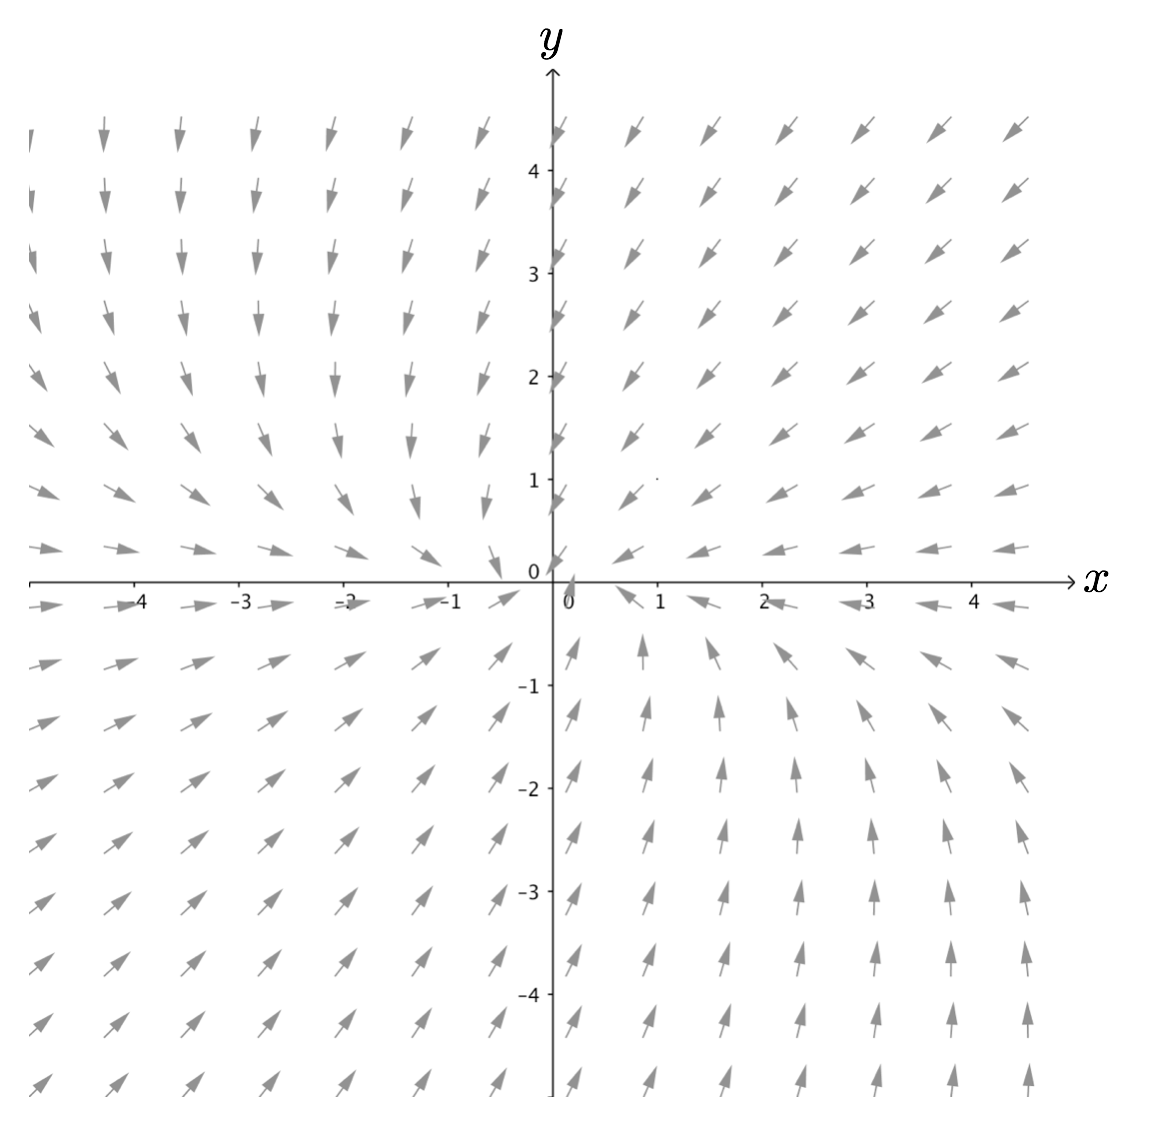
\includegraphics[width=2.5in]{11/11HWVectorField1.png}
%\item[(B)] 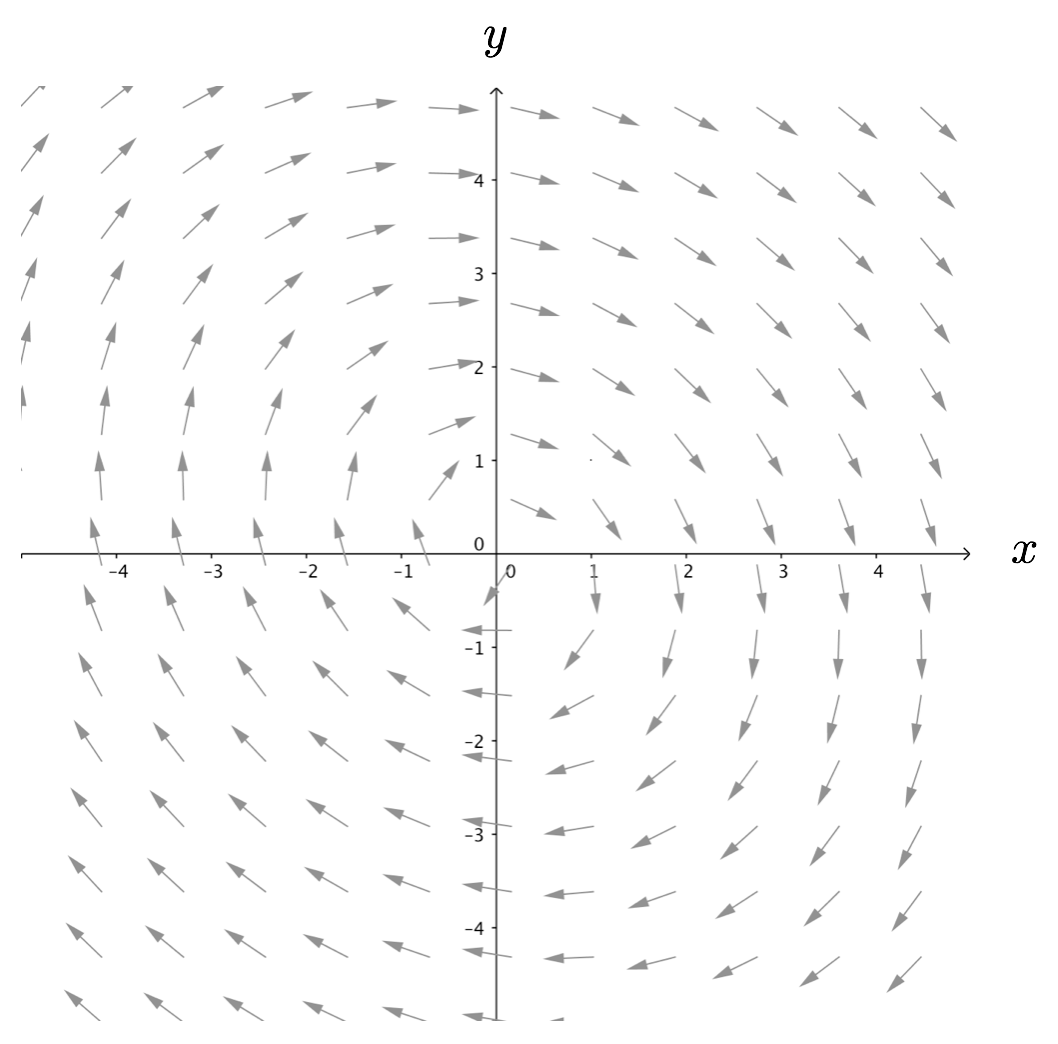
\includegraphics[width=2.5in]{11/11HWVectorField2.png} \\
%\item[(C)] 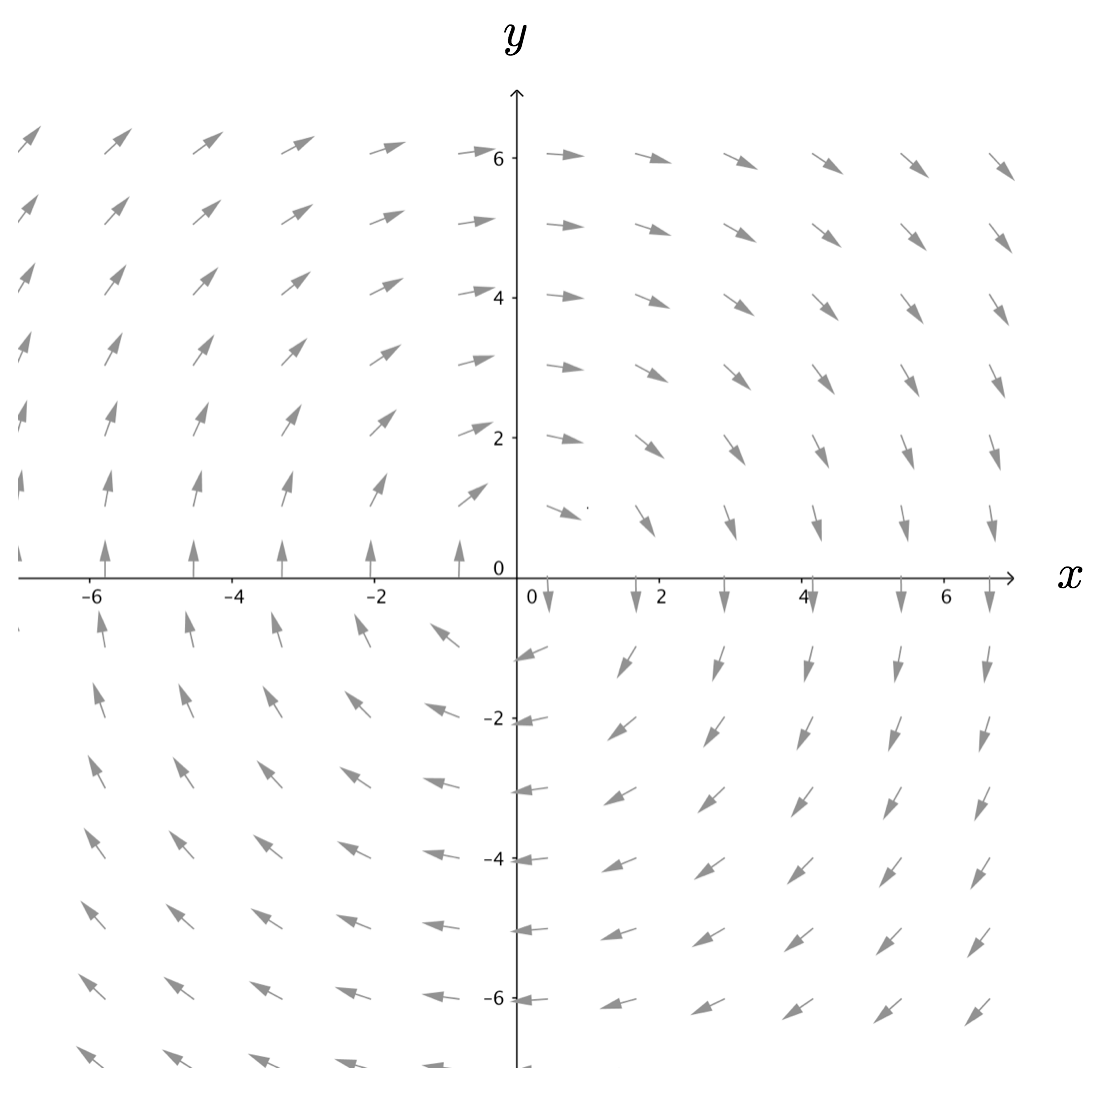
\includegraphics[width=2.5in]{11/11HWVectorField3.png}
%\item[(D)] 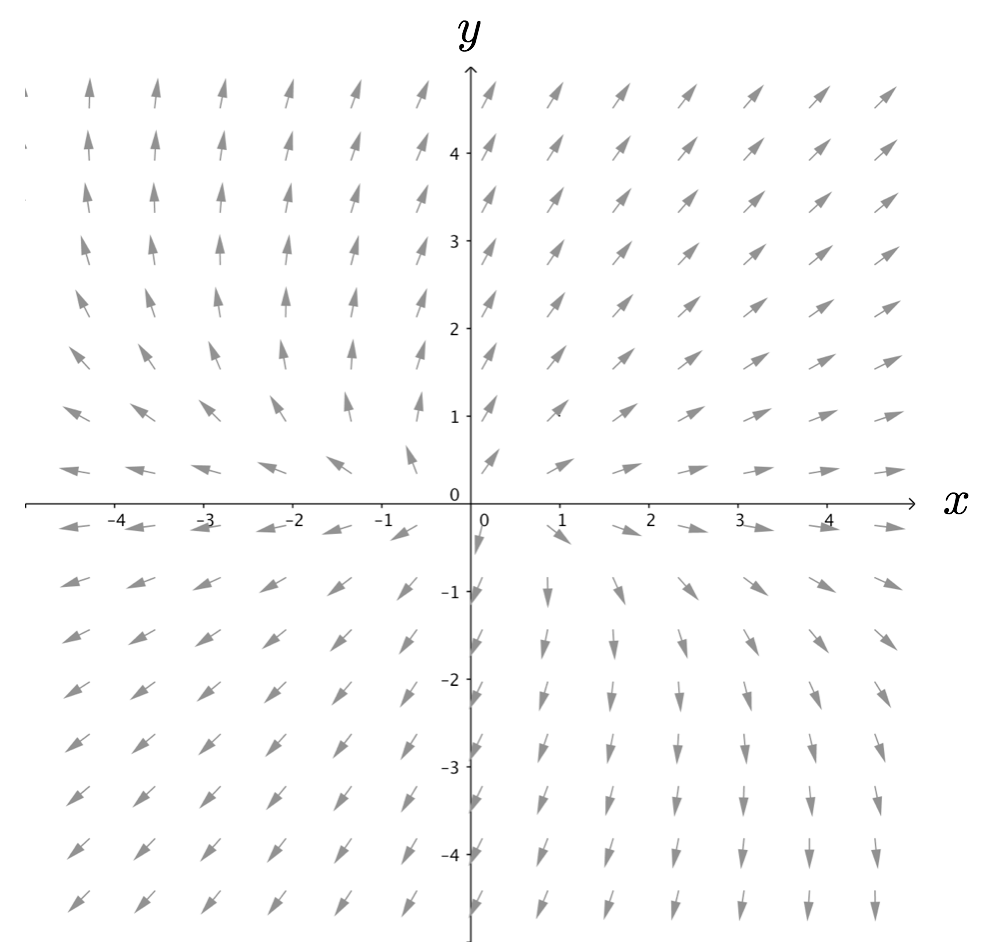
\includegraphics[width=2.5in]{11/11HWVectorField4.png}
%\end{enumerate*}
%
%For each sentence below, fill in the blank with choices from the following two lists:
%
%\begin{center}
%\begin{tabular}{ccccc}
%\textbf{\underline{Spring System (First Blank)}} &&& \textbf{\underline{Solutions (Second Blank)}} \\
%a damped spring &&& $c_1\cos(t) + c_2\sin(t)$ \\
%an overdamped spring &&& $e^{-t}(c_1\cos(t) + c_2\sin(t))$ \\
%an undamped spring &&& $e^{t}(c_1\cos(t) + c_2(\sin(t))$ \\
%something other than a spring &&& $c_1 e^t + c_2 e^{2t}$ \\
%&&& $c_1 e^{-t} + c_2 e^{-2t}$ \\
%&&& $c_1 e^{-t} + c_2 e^{2t}$ \\
%&&& $c_1 e^t + c_2 e^{-2t}$	
%\end{tabular}
%\end{center}
%
%Phase plane (A) corresponds to \rule{1in}{.5pt} and the solutions look like $x(t)$=\rule{1.5in}{.5pt} \\
%
%Phase plane (B) corresponds to \rule{1in}{.5pt} and the solutions look like $x(t)$=\rule{1.5in}{.5pt} \\
%
%Phase plane (C) corresponds to \rule{1in}{.5pt} and the solutions look like $x(t)$=\rule{1.5in}{.5pt} \\
%
%Phase plane (D) corresponds to \rule{1in}{.5pt} and the solutions look like $x(t)$=\rule{1.5in}{.5pt}
%
%\clearpage
%
%\item What type of system (undamped, damped, overdamped) do the following best correspond to? Explain your reasoning. \label{11HWproblem5}
%\begin{enumerate}
%\item A car that bounces every time it hits a bump
%\item A pendulum immersed in a vat of honey
%\item A bungee jumper
%\end{enumerate}
%
%\item In each part, write a differential equation corresponding to the given scenario: \label{11HWproblem6}
%\begin{enumerate}
%\item An undamped spring
%\item An underdamped spring
%\item An overdamped spring
%\end{enumerate}
%
%\item Does Adding Solutions Always Result in Another Solution? \\
%
%In deriving the general solution to the spring mass problem, two solutions were added to get another solution. This worked for the particular equations at hand, but does adding two solutions to a system of differential equations of the form    
%\begin{align*}
%\frac{dx}{dt}&=ax+by\\ \frac{dy}{dt}&= cx+dy
%\end{align*}
% always result in another solution to the same system of differential equations? Below is a proof that this in fact is true.
%
%\noindent \underline{Claim}:
%If  $\displaystyle \begin{pmatrix}
%x_1(t)\\y_1(t)
%\end{pmatrix}$  and $\displaystyle \begin{pmatrix}
%x_2(t)\\y_2(t)
%\end{pmatrix}$  are solutions (not necessarily straight line solutions) to a system of differential equations of the form  \begin{align*}\begin{split}
%\frac{dx}{dt}&=ax+by\\ \frac{dy}{dt}&= cx+dy
%\end{split}\end{align*}
% then the sum of these two solutions is also a solution. That is, if we call the sum of these two solutions  $\displaystyle \begin{pmatrix} x_3(t)\\y_3(t) \end{pmatrix}$ where 
% \[ \begin{pmatrix}
%x_3(t)\\y_3(t)
%\end{pmatrix}=\begin{pmatrix}
%x_1(t)\\y_1(t)
%\end{pmatrix}+\begin{pmatrix}
%x_2(t)\\y_2(t)
%\end{pmatrix}=\begin{pmatrix}
%x_1(t)+x_2(t)\\y_1(t)+y_2(t)
%\end{pmatrix},\]
% then  $\displaystyle \begin{pmatrix} x_3(t)\\y_3(t) \end{pmatrix}$  is also a solution to the same system of differential equations.  
%
%\noindent\underline{Proof:}
%In order to show that $\displaystyle \begin{pmatrix} x_3(t)\\y_3(t) \end{pmatrix}$  is a solution, we need to verify it satisfies the system of differential equations. This is, we need to show that  
%\begin{align*}\begin{split}
%\frac{d}{dt}x_3(t)&=ax_3(t)+by_3(t)\\ \frac{d}{dt}y_3(t)&= cx_3(t)+dy_3(t)
%\end{split}.\end{align*}
%
%Since   
%\[ \begin{pmatrix}
%x_3(t)\\y_3(t)\end{pmatrix}=\begin{pmatrix}
%x_1(t)+x_2(t)\\y_1(t)+y_2(t)
%\end{pmatrix},\] we know that   
%\begin{align}\begin{split}
%\frac{d}{dt}x_3(t)&=\frac{d}{dt}x_1(t)+\frac{d}{dt}x_2(t)\\ \frac{d}{dt}y_3(t)&= \frac{d}{dt}y_1(t)+\frac{d}{dt}y_2(t) 
%\end{split}.\label{12HWeqn1}\end{align}
%Because $\displaystyle \begin{pmatrix} x_1(t)\\y_1(t) \end{pmatrix}$   is a solution, it satisfies the system of differential equations. That is,    
%\begin{align}\begin{split}
%\frac{d}{dt}x_1(t)&=ax_1(t)+by_1(t)\\ \frac{d}{dt}y_1(t)&= cx_1(t)+dy_1(t) \label{12HWeqn2}
%\end{split}\end{align}  
%Similarly, since   $\displaystyle \begin{pmatrix} x_2(t)\\y_2(t) \end{pmatrix}$   is a solution,  
%  
%\begin{align}\begin{split}
%\frac{d}{dt}x_2(t)&=ax_2(t)+by_2(t)\\ \frac{d}{dt}y_2(t)&= cx_2(t)+dy_2(t) \label{12HWeqn3}
%\end{split}\end{align}  
%
%Substituting \eqref{12HWeqn2} and \eqref{12HWeqn3} into \eqref{12HWeqn1} yields 
%\begin{align*}\begin{split}
%\frac{d}{dt}x_3(t)&=ax_1(t)+by_1(t)+ax_2(t)+by_2(t)\\ \frac{d}{dt}y_3(t)&= cx_1(t)+dy_1(t)+cx_2(t)+dy_2(t) 
%\end{split}.\end{align*}  
%Rearranging terms yields
%\begin{align*}\begin{split}
%\frac{d}{dt}x_3(t)=ax_1(t)+ax_2(t)+by_1(t)+by_2(t) &= a[x_1(t)+x_2(t)]+b[y_1(t)+y_2(t)] \\ \frac{d}{dt}y_3(t)= cx_1(t)+cx_2(t)+dy_1(t)+dy_2(t) &= c[x_1(t)+x_2(t)]+d[y_1(t)+y_2(t)] 
%\end{split}.\end{align*}  
%
%
%Finally, using the fact that   \[ \begin{pmatrix}
%x_3(t)\\y_3(t)\end{pmatrix}=\begin{pmatrix}
%x_1(t)+x_2(t)\\y_1(t)+y_2(t)
%\end{pmatrix},\]   yields \begin{align*}\begin{split}
%\frac{d}{dt}x_3(t)&=ax_3(t)+by_3(t)\\ \frac{d}{dt}y_3(t)&= cx_3(t)+dy_3(t)
%\end{split}\end{align*}
%   which is what we set out to show. Therefore $\displaystyle  \begin{pmatrix}
%x_3(t)\\y_3(t)\end{pmatrix}$  is also a solution to the system of differential equations.
%
%\clearpage
%
%\begin{enumerate}
%\item	Suppose that \label{12HWprob7parta} $\displaystyle  \begin{pmatrix}
%x_1(t)\\y_1(t)\end{pmatrix}$  and $\displaystyle  \begin{pmatrix}
%x_2(t)\\y_2(t)\end{pmatrix}$  are solutions to the system of differential equations
%\begin{align*}\begin{split}
%\frac{dx}{dt}&=ax+by+1\\ \frac{dy}{dt}&= cx+dy+2
%\end{split}\end{align*}
% where $a, b, c,$ and $d$ are constants. Josh claims that the sum of these two solutions is also a solution to the same system of differential equations. Do you agree with his claim? Either develop a similar proof as above to support this claim or point to where (and why) the above proof fails.
%
%\item	Suppose that \label{12HWprob7partb} $\displaystyle  \begin{pmatrix}
%x_1(t)\\y_1(t)\end{pmatrix}$  and $\displaystyle  \begin{pmatrix}
%x_2(t)\\y_2(t)\end{pmatrix}$  are solutions to the system of differential equations
%\begin{align*}\begin{split}
%\frac{dx}{dt}&=ax^2+by\\ \frac{dy}{dt}&= cx+dy
%\end{split}\end{align*}
% where $a, b, c,$ and $d$ are constants. Angela claims that the sum of these two solutions is also a solution to the same system of differential equations. Do you agree with her claim? Either develop a similar proof as above to support this claim or point to where (and why) the above proof fails.
%
%\end{enumerate}

%\end{enumerate}
